\chapter{Caso de estudio: Sistema de climatización}
\label{chap:caso_estudio}

Para verificar la arquitectura definida, decidimos implementar un pequeño sistema autoadaptativo. Se trata de un sistema de climatización, que gestiona la temperatura de una habitación. Para ello, dispondremos de un aire acondicionado, que calentará o enfriará la habitación según corresponda.

\section{Análisis}

El primer paso es capturar los requisitos del sistema a implementar. Cómo hemos comentado, queremos desarrollar un sistema de climatización. Este sistema regulará la temperatura de una habitación mediante el uso de un aparato de aire acondicionado.

El aparato de aire acondicionado ofrece tres modos de funcionamiento: un modo para calentar la estancia, otro para enfriarla, y un estado neutral (apagado). Además, lo hemos dotado con un termómetro interno que nos reporta la temperatura periódicamente.

Para poder climatizar la habitación, necesitamos que el usuario defina su temperatura objetivo: la temperatura de confort. Cambios en la temperatura deberán activar o desactivar el aparato para mantenerla.

Además, nos interesa evitar que el aire acondicionado se encienda y se apague constantemente cuando se alcance o sobrepase esta temperatura. Por ello, definimos unas temperaturas umbrales, tanto de frío como de calor, a partir de las cuales se encenderá el aparato.

\section{Diseño}

Del análisis anterior ya podemos deducir la existencia de dos componentes: un aparato de aire acondicionado (el sistema gestionado) y un termómetro (la sonda). Aparte de ellos, deberemos implementar la infraestructura necesaria para comunicarse con nuestro bucle MAPE-K: monitores, módulos de reglas y efectores que nos permitan interactuar con el sistema manejado.

Para describir el diseño usaremos la notación de sistemas autoadaptativos descrita en \cite{fonsEspecificacionSistemasAutoadaptativos2021}.

\subsection{Sondas:}

Para implementar el sistema, requerimos de las siguientes sondas:

\begin{longtable}{|r p{11.5cm}|}
    \hline
    \textbf{Sonda:} & \emph{thermometer}  \\
    \textbf{Descripción:} & Reporta la temperatura actual de la habitación (en ºc). \\
    \textbf{Monitor:} & \emph{Climatisation.Monitor} \\
    \textbf{Datos:} & \emph{temperature} \\
    \hline
    \textbf{Sonda:} & \emph{airconditioner-mode-changed-probe}  \\
    \textbf{Descripción:} & Reporta el modo de funcionamiento del aire acondicionado cuando este cambia. \\
    \textbf{Monitor:} & \emph{Climatisation.Monitor} \\
    \textbf{Datos:} & \emph{airconditioner-mode} \\
    \hline
    \textbf{Sonda:} & \emph{airconditioner-adaption-loop-registration}  \\
    \textbf{Descripción:} & Cuando arranca el servicio de aire acondicionado, registra la configuración inicial del sistema. \\
    \textbf{Monitor:} & \emph{Climatisation.Monitor} \\
    \textbf{Datos:} & \emph{airconditioner.is-deployed}, \emph{airconditioner-mode}, \emph{target-temperature}, \emph{cold-temperature-threshold}, \emph{hot-temperature-threshold} \\
    \hline

    \caption{Sondas del sistema de climatización.}
    \label{tab:climatisation-probes}
\end{longtable}

\subsection{Propiedades de adaptación:}

También podemos deducir cuáles son nuestras propiedades de adaptación:

\begin{longtable}{|r p{11.5cm}|}
    \hline
    \textbf{Propiedad:} & \emph{temperature}  \\
    \textbf{Descripción:} & Representa la temperatura actual de la habitación (en ºC).  \\
    \textbf{Tipo de dato:} & \emph{float} \\
    \hline
    \textbf{Propiedad:} & \emph{target-temperature}  \\
    \textbf{Descripción:} & La temperatura de confort definida por el usuario. El sistema deberá adaptarse para alcanzarla.  \\
    \textbf{Tipo de dato:} & \emph{float} \\
    \hline
    \textbf{Propiedad:} & \emph{cold-temperature-threshold}  \\
    \textbf{Descripción:} & La temperatura umbral de frío (en ºc). Si la temperatura baja por debajo de este umbral, deberá calentarse la habitación. \\
    \textbf{Tipo de dato:} & \emph{float} \\
    \hline
    \textbf{Propiedad:} & \emph{hot-temperature-threshold}  \\
    \textbf{Descripción:} & La temperatura umbral de calor (en ºc). Si la temperatura sube por encima de este umbral, deberá enfriarse la habitación. \\
    \textbf{Tipo de dato:} & \emph{float} \\
    \hline
    \textbf{Propiedad:} & \emph{airconditioner.is-deployed}  \\
    \textbf{Descripción:} & Indica si el servicio de aire acondicionado está desplegado y en funcionamiento.  \\
    \textbf{Tipo de dato:} & \emph{bool} \\
    \hline
    \textbf{Propiedad:} & \emph{airconditioner-mode}  \\
    \textbf{Descripción:} & Representa el modo de operación actual del aire acondicionado: \emph{Off} = 0, \emph{Cooling} = 1, \emph{Heating} = 2  \\
    \textbf{Tipo de dato:} & Enumerado \\
    \hline

  \caption{Propiedades de adaptación del sistema de climatización.}
  \label{tab:climatisation-adaption-properties}
\end{longtable}

\subsection{Monitores:}

Necesitaremos definir varios monitores para capturar los datos de las sondas. En algunos casos, para evitar falsos positivos, y que se lleve a cabo adaptaciones provocadas por errores de medición, deberemos filtrar estos datos.

Por ejemplo, en el monitor de las temperaturas, \emph{climatisation.monitor.temperature}. Como en el ejemplo trabajamos con un aire acondicionado ficticio, le hemos establecido un margen de error grande: Si la nueva medida de temperatura está a 5ºc de diferencia o más, y hay menos de un minuto de diferencia entre ellas; la descartaremos. De esta forma, evitamos que el aire acondicionado se active o desactive por un error de medición.

\begin{longtable}{|p{3.7cm} p{10.7cm}|}
    \hline

    \textbf{Monitor:} & \emph{climatisation.monitor.temperature}  \\
    \textbf{Descripción:} & Recibe los reportes de temperatura de los termómetros. También filtra estos datos para detectar casos donde se sospecha un error de lectura. \\
    \textbf{Afecta a propiedades de adaptación:} & \emph{temperature} \\
    \multirow{3}*{\textbf{Acciones:}}
        & \textbf{SI} |\emph{new-temperature} - \emph{temperature}| <= 5.0 \\
        & \textbf{O} request.DateTime - previousMeasurement.DateTime > 60s \\
        & \textbf{ACTUALIZA-KNOWLEDGE} \emph{temperature} = \emph{new-temperature} \\
    \hline

    \textbf{Monitor:} & \emph{climatisation.monitor.configuration}  \\
    \textbf{Descripción:} & Recibe la configuración del aire acondicionado y la registra en el \emph{knowledge}. \\
    \textbf{Afecta a propiedades de adaptación:} & \emph{airconditioner.is-deployed}, \emph{airconditioner-mode}, \emph{target-temperature}, \emph{cold-temperature-threshold}, \emph{hot-temperature-threshold} \\
    \multirow{2}*{\textbf{Acciones:}}
        & \textbf{SI} \emph{property} != \emph{new-value} \\
        & \textbf{ACTUALIZA-KNOWLEDGE} \emph{property} = \emph{new-value} \\
    \hline

  \caption{Monitores del bucle MAPE-K del sistema de climatización.}
  \label{tab:climatisation-monitors}
\end{longtable}

\subsection{Reglas de adaptación}
\label{sec:caso-estudio-diseño-reglas}

En base a cambios de la temperatura local, deberemos decidir si es necesario llevar a cabo una acción correctiva. Por ejemplo, que si la temperatura es inferior al umbral de temperatura fría, el aparato se enciende en modo calentador. Para ello, deberemos implementar un servicio de reglas (\emph{Climatisation.Rules.Service}). En él, incluiremos una serie de reglas que se disparen cuando cambie una de nuestras propiedades de adaptación. En este caso, la temperatura.

Como comentamos en el capitulo anterior, en nuestro ejemplo de bucle MAPE-K, nos limitamos a implementar las adaptaciones de tipo set-parameter. Por tanto, no tendremos reglas de despliegue o de binding.

En la tabla \ref{tab:adaption-rules-climatisation} definimos las cuatro reglas necesarias:

\begin{longtable}{|r p{12.8cm}|}
    \hline
    \textbf{Regla:} & \emph{EnableAirConditionerHeatingModeWhenColdTemperatureThresholdExceeded}  \\
    \textbf{Descripción:} & Activa el aire acondicionado en modo calefacción cuando la temperatura sea inferior al umbral de frío.  \\
    \textbf{Condición:} & \emph{airconditioner-mode} != \emph{Heating} \textbf{AND} \emph{temperature} <= \emph{cold-temperature-threshold}  \\
    \textbf{Cuerpo:}   &  \\
    & 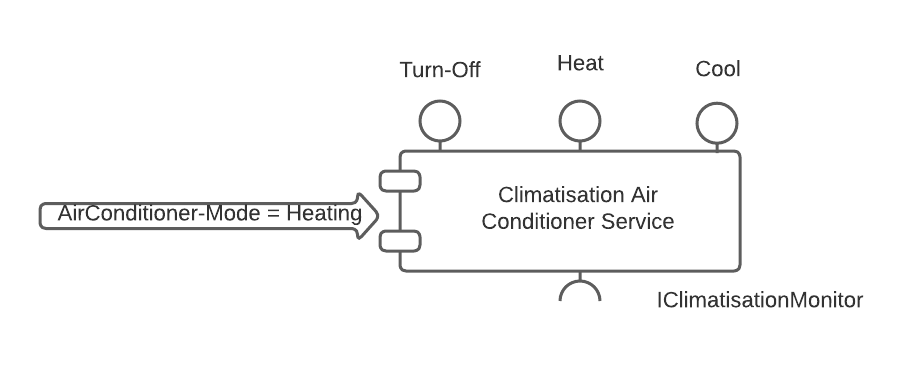
\includegraphics[scale=0.75]{cap_caso-estudio/images/adaption-loop-rule-heat} \\
    \hline

    \textbf{Regla:} & \emph{DisableAirConditionerWhenHeatingModeEnabledAndTargetTemperatureAchieved}  \\
    \textbf{Descripción:} & Apaga el aire acondicionado cuando el modo calefacción está activo y se ha alcanzado la temperatura de confort.  \\
    \textbf{Condición:} & \emph{airconditioner-mode} == \emph{Heating} \textbf{AND} \emph{temperature} >= \emph{target-temperature}  \\
    \textbf{Cuerpo:} &  \\
    & 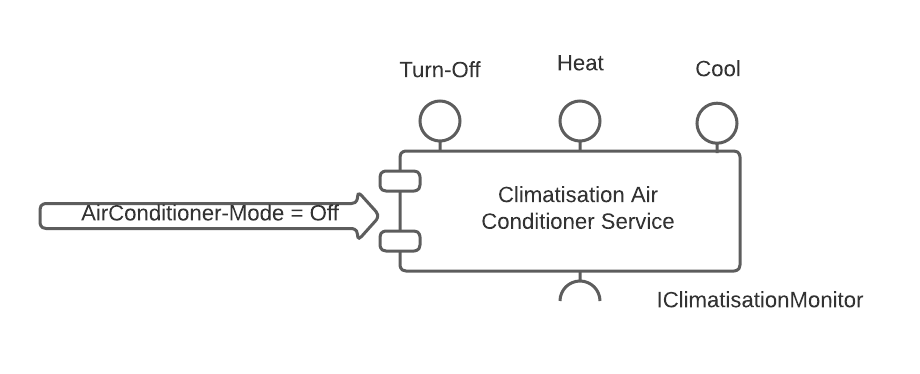
\includegraphics[scale=0.75]{cap_caso-estudio/images/adaption-loop-rule-off} \\
    \hline

    \textbf{Regla:} & \emph{EnableAirConditionerCoolingModeWhenTemperatureThresholdExceeded}  \\
    \textbf{Descripción:} & Activa el aire acondicionado en modo enfriar cuando la temperatura sea superior al umbral de calor.  \\
    \textbf{Condición:} & \emph{airconditioner-mode} != \emph{Cooling} \textbf{AND} \emph{temperature} >= \emph{hot-temperature-threshold}  \\
    \textbf{Cuerpo:} &  \\
    & 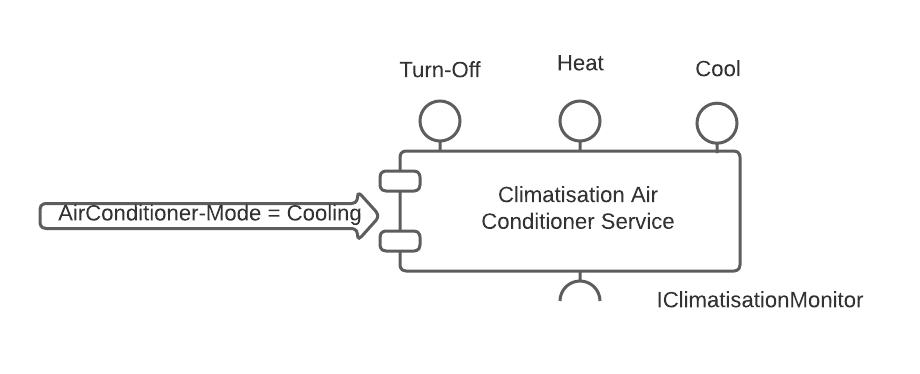
\includegraphics[scale=0.75]{cap_caso-estudio/images/adaption-loop-rule-cooling} \\
    \hline

    \textbf{Regla:} & \emph{DisableAirConditionerWhenCoolingAndTargetTemperatureAchievedAdaptionRule}  \\
    \textbf{Descripción:} & Apaga el aire acondicionado cuando el modo enfiar está activo y se ha alcanzado la temperatura de confort.  \\
    \textbf{Condición:} & \emph{airconditioner-mode} == \emph{Cooling} \textbf{AND} \emph{temperature} <= \emph{target-temperature}  \\
    \textbf{Cuerpo:} &  \\
    & 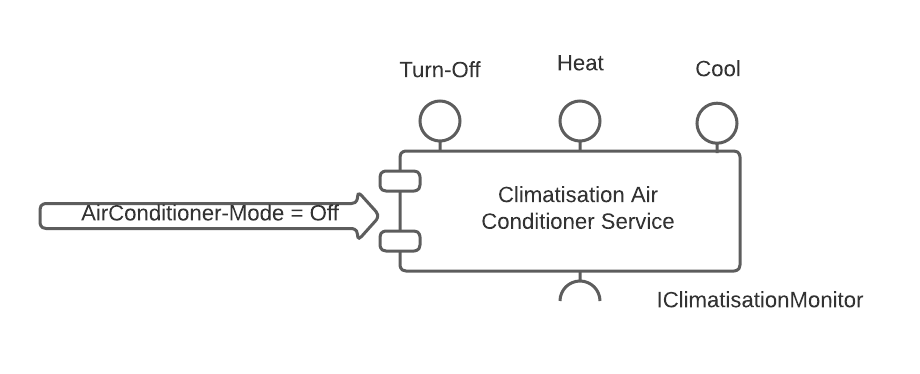
\includegraphics[scale=0.75]{cap_caso-estudio/images/adaption-loop-rule-off} \\
    \hline

  \caption{Reglas de adaptación del sistema de climatización.}
  \label{tab:adaption-rules-climatisation}
\end{longtable}

\subsection{Efectores:}

Una vez se evaluén estas reglas, solicitamos un cambio en la configuración del sistema. El módulo de planificación comprobará contra el conocimiento y el estado actual del sistema cuáles de los cambios solicitados es necesario aplicar. Si por ejemplo la propiedad ya tiene el valor solicitado, no hará falta ejecutarla.

El modulo de ejecución recibirá la petición y se la redirigirá a los efectores del sistema de climatización. En este caso, requerimos de efectores que cambien el modo del aire acondicionado según corresponda.

\begin{table}[htb]
  \centering

  \begin{tabular}{|r p{11.5cm}|}
    \hline
    \textbf{Efector:} & \emph{airconditioner.heat}  \\
    \textbf{Descripción:} & Activa el modo calentar del aire acondicionado. \\
    \hline
    \textbf{Efector:} & \emph{airconditioner.cool}  \\
    \textbf{Descripción:} & Activa el modo enfriar del aire acondicionado. \\
    \hline
    \textbf{Efector:} & \emph{airconditioner.turn-off}  \\
    \textbf{Descripción:} & Apaga el aire acondicionado. \\
    \hline
  \end{tabular}

  \caption{Efectores del sistema de climatización.}
    \label{tab:climatisation-effectors}
\end{table}

Hecho esto, el sistema se adapta a a la nueva situación, y reportará una nueva temperatura en cuanto corresponda. La temperatura variará dependiendo de si está apagado o no.

\subsection{Configuración del sistema}

Requerimos entonces 4 servicios para implementar la solución: Servicio de aire acondicionado, monitor de climatización, el servicio de reglas y el servicio de efectores. Con ellos, podemos adaptarnos al bucle MAPE-K descrito en el capítulo %TODO: Capítulo.

\section{Implementación}

Para la implementación, hemos utilizado las mismas tecnologías descritas en el capítulo \ref{chap:implementación}: microservicios \texttt{ASP.NET}, comunicación mediante APIs REST y \foreign{english}{brokers} de mensajería \texttt{RabbitMQ}. Generamos los API Clients con OpenAPI y demás.

A continuación describiremos todos los servicios implementados:

\subsection{Servicio de aire acondicionado}

El servicio de aire acondicionado será nuestro sistema manejado. Como no disponemos de un aire acondicionado real, hemos optado por implementar uno ficticio. Este cuenta con tres estados de operación: apagado (\texttt{OFF}), enfriando (\texttt{COOLING}) o calentando (\texttt{HEATING}). Según el modo, aumentará o disminuirá la temperatura que reporta un termómetro interno. Además, cuando está apagado, la temperatura ficticia aumenta o disminuye gradualmente según una configuración. De esta forma, podemos simular los cambios de temperatura más rápido y ver si se aplican correctamente las adaptaciones correspondientes.

Además, este servicio expone tres endpoints HTTP, que nos permiten cambiar el modo del aire acondicionado. Serán estos los que invocará el servicio de efectores para manipular su estado.

Por otro lado, para simplificar la configuración del sistema, optamos por registrar las propiedades del aire acondicionado durante su arranque. Tenemos para ello un servicio en segundo plano (un \foreign{english}{background service} de \texttt{ASP.NET}) que registra la configuración inicial durante el arranque. Así le daremos valor a las propiedades como los umbrales de temperatura o las variables como is-deployed. \textcolor{red}{Es necesario un fragmento de código?}

\subsection{Monitor}

El monitor de la solución expone endpoints para recabar las mediciones de las sondas. En este caso, las mediciones de temperatura del aire acondicionado: \texttt{POST Measurement/Temperature}. Este endpoint recibe la temperatura y ejecuta las validaciones descritas en el apartado anterior: descarta valores con diferencias de 5ºC tomados en menos de un minuto, entre otras. Si el valor es válido, lo manda al servicio de monitorización. A su vez este lo almacenará en el conocimiento como propiedad de adaptación.

El servicio también ofrece endpoints para actualizar la configuración del aire acondicionado en el conocimiento. Así podrá registrar su configuración inicial o los modos de operación cuando cambien. Son un subconjunto de los endpoints que ofrece el conocimiento, expuestos a través del servicio de monitorización del bucle.

\subsection{Reglas}

En cuanto al servicio de reglas, este contiene las cuatro reglas definidas en el apartado \ref{sec:caso-estudio-diseño-reglas}. Estas activan o desactivan el aire acondicionado en base a la temperatura de la estancia. Se han implementado siguiendo la estructura descrita en el apartado \ref{sec:implementacion-modulo-reglas}. Todas ellas heredan de las clase abstracta \texttt{AdaptionRuleBase}. Deben implementar los métodos para evaluar la condición y ejecutar su acción; y deben declarar las propiedades de adaptación de las que dependen.

Para describirlas, nos centraremos en la regla \texttt{Disable Air Conditioner When Cooling And Target Temperature Achieved Adaption Rule}. Esta desactiva el aire acondicionado cuando está en modo enfriamiento y se ha alcanzado la temperatura de enfriamiento de la estancia. A lo largo de la memoria ya habíamos mostrado algunos fragmentos de código de esta.

Las reglas describen las propiedades o configuraciones de las que dependen mediante atributos. Se trata de aquellas que requiere para evaluar su condición. Tomemos por ejemplo el fragmento \ref{ls:adaption-rule-dependencies}. Observamos que declara de tres dependencias: \texttt{airconditioner-mode}, \texttt{temperature} y \texttt{hot-temperature-threshold}.

En cuanto a la implementación, ya habíamos mostrado su método \texttt{Execute} en el fragmento \ref{ls:change-request-builder}. Solo nos queda exponer la implementación de referencia del método \texttt{Evaluate Condition}. En el fragmento \ref{ls:adaption-rule-evaluate-condition} ofrecemos la implementación de la condición \emph{airconditioner-mode} == \emph{Cooling} \textbf{AND} \emph{temperature} <= \emph{target-temperature}. Observamos que en las líneas 3-5, 12-15 y 17-20 se obtienen las propiedades de adaptación o claves de configuración desde el servicio de análisis. En base a ellas, en las líneas 22-23 se evalúa la condición descrita.

\begin{lstlisting}[language={[Sharp]C},caption={Implementación de referencia del método \texttt{EvaluateCondition}. La regla obtiene del conocimiento el estado actual del sistema y determina si debe ejecutarse.},captionpos=b, label=ls:adaption-rule-evaluate-condition]
protected override async Task<bool> EvaluateCondition()
{
  var currentTemperature =
    await _propertyService.GetProperty<TemperatureMeasurementDTO>(
      ClimatisationConstants.Property.Temperature);

  if (currentTemperature is null)
  {
      return false;
  }

  var airConditionerMode = await _configurationService
    .GetConfigurationKey<AirConditioningMode?>(
        ClimatisationAirConditionerConstants.AppName,
        ClimatisationAirConditionerConstants.Configuration.Mode);

  var targetTemperature = await _configurationService
      .GetConfigurationKey<float?>(
        ClimatisationAirConditionerConstants.AppName,
        ClimatisationConstants.Configuration.TargetTemperature);

  return airConditionerMode == AirConditioningMode.Cooling
      && currentTemperature.Value <= targetTemperature;
}
\end{lstlisting}

\subsection{Efectores}

Finalmente, tenemos el servicio de efectores. En la última etapa del bucle de adaptación, el módulo de ejecución emite una notificación con las acciones de adaptación que debe ejecutarse para determinado componente del sistema manejado. El servicio de efectores se suscribirá a estas notificaciones de aquellos componentes que gestiona. En este caso, las referentes al aire acondicionado.

Una vez capturada, determinará el tipo de acción que debe ejecutar e invocará a su implementación. En nuestro caso, hacemos un dispatch interno del evento

Para el caso de estudio, por restricciones de tiempo, nos limitamos a implementar las adaptaciones que implicaban cambios en la configuración del sistema manejado (adaptaciones \foreign{english}{set parameter}). La implementación del componente manejado determinará cómo se ejecutarán estas acciones. Dependemos de los efectores que expongan. Por ejemplo, para el servicio de aire acondicionado, cambiar el modo de operación supone invocar a unos endpoints que expone. Por ejemplo: (\texttt{POST /airconditioner/turn-off}).

\begin{lstlisting}[language={[Sharp]C},caption={Implementación de los efectores del aire acondicionado. Invocan a los endpoints HTTP en base a las acciones de adaptación.},captionpos=b, label=ls:effector-airconditioner-set-parameter]
public async Task<Unit> Handle(
  SetAirConditionerModeRequest notification,
  CancellationToken cancellationToken)
{
    var succeeded = Enum.TryParse(
      notification.Value,
      out AirConditioningMode mode);

    if (!succeeded)
    {
        return Unit.Value;
    }

    switch (mode)
    {
        case AirConditioningMode.Off:
            await _airConditionerApi.AirConditionerTurnOffPostAsync(cancellationToken);
            break;

        case AirConditioningMode.Cooling:
            await _airConditionerApi.AirConditionerCoolPostAsync(cancellationToken);
            break;

        case AirConditioningMode.Heating:
            await _airConditionerApi.AirConditionerHeatPostAsync(cancellationToken);
            break;
    }

    return Unit.Value;
}
\end{lstlisting}

\section{Despliegue y Pruebas}

Debido a la gran cantidad de microservicios que componen la solución, optamos por empaquetarlos en contenedores \texttt{Docker}. Para ello, definimos un plan de despliegue con Docker Compose, que nos permitía definir el número de instancias y las dependencias entre ellas. Por ejemplo, todos los servicios que requieran de un bus de mensajería, dependen de la instancia de RabbitMQ desplegada. Por simplicidad, optamos por desplegar una única instancia para toda la solución. Lo ideal sería que cada que requiriera de emitir sus propias notificaciones dispongan de la suya propia, que se adapte más a sus necesidades.

\subsection{Telemetría}

Un punto en el que queremos hacer hincapié es en la telemetría. Debido a que estamos tratando con un sistema distribuido es complicado conocer el estado del sistema en determinado momento. Especialmente en este caso, que participan más de diez servicios distintos.

Por defecto, solo contábamos con los \emph{logs} de consola, que mostramos en la figura \ref{fig:console-logs}. Aparecen en una única ventana intercalados los registros de todos los servicios. Aunque nos pueden resultar útil, es una aproximación ineficiente y según aumente la escala de peticiones simultáneamente se volverá más difícil de interpretar.

\begin{figure}[h]
  \centering
  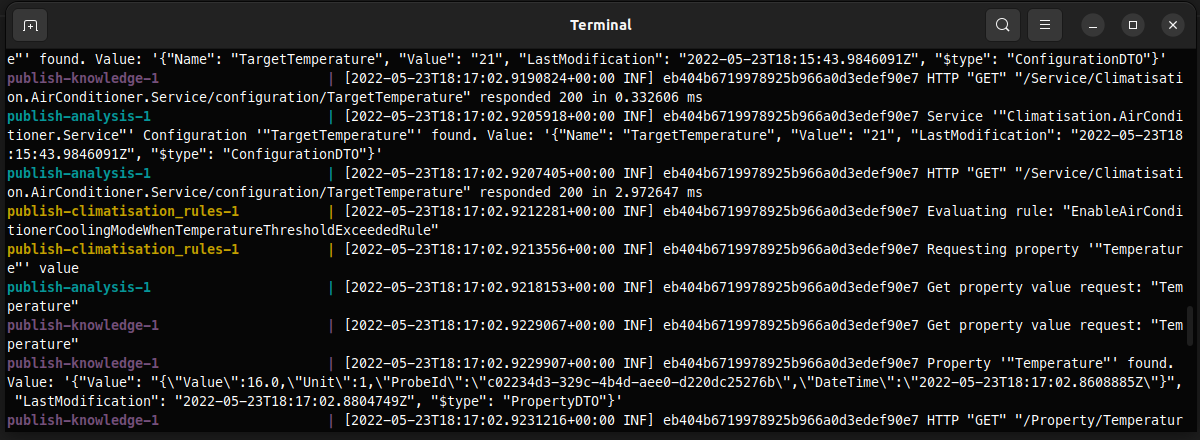
\includegraphics[scale=1.45]{cap_caso-estudio/images/console-logs}
  \caption{Extracto de \emph{logs} de una ejecución habitual.}
  \label{fig:console-logs}
\end{figure}

Por ello, para que resultara más sencillo trabajar en la implementación de los servicios y diagnosticar qué ocurre con el sistema, decidimos implementar una solución de observabilidad. La observabilidad es \cite{parkerProblemDistributedTracing2020} y consta de tres partes distintas: %TODO CITA
\begin{itemize}
  \item \textbf{Logs}: \textcolor{red}{A recording of an Event. Typically the record includes a timestamp indicating when the Event happened as well as other data that describes what happened, where it happened, etc. \cite{opentelemetryOpenTelemetryDocumentation2022} Provide extremely fine-grained detail on a given service, but have no built-in way to provide that detail in the context of a request. \cite{parkerProblemDistributedTracing2020}}
  \item \textbf{Métricas}: \textcolor{red}{Son agregados que nos permiten conocer el estado de las estancias de nuestros servicios. Records a data point, either raw measurements or predefined aggregation, as timeseries with Metadata. \cite{opentelemetryOpenTelemetryDocumentation2022}}
  \item \textbf{Trazas distribuidas}: \textcolor{red}{Tracks the progression of a single Request, called a Trace, as it is handled by Services that make up an Application. A Distributed Trace transverses process, network and security boundaries. \cite{opentelemetryOpenTelemetryDocumentation2022}  providing visibility into the operation of your microservice architecture. It allows you to gain critical insights into the performance and status of individual services as part of a chain of requests in a way that would be difficult or time-consuming to do otherwise. Distributed tracing gives you the ability to understand exactly what a particular, individual service is doing as part of the whole, enabling you to ask and answer questions about the performance of your services and your distributed system. \cite{parkerProblemDistributedTracing2020}}
\end{itemize}

Para poder capturar todos estos elementos, optamos por usar el estándar OpenTelemetry. Se trata de una librería estándar utilizada para instrumentar el código de las aplicaciones. Distintas compañías del ámbito de la telemetría software ofrecen APIs que capturan el output de esta librería.

Gracias a él pudimos capturar la telemetría de la siguiente forma implementar usando tres servicios distintos:

\begin{figure}[h]
  \centering
  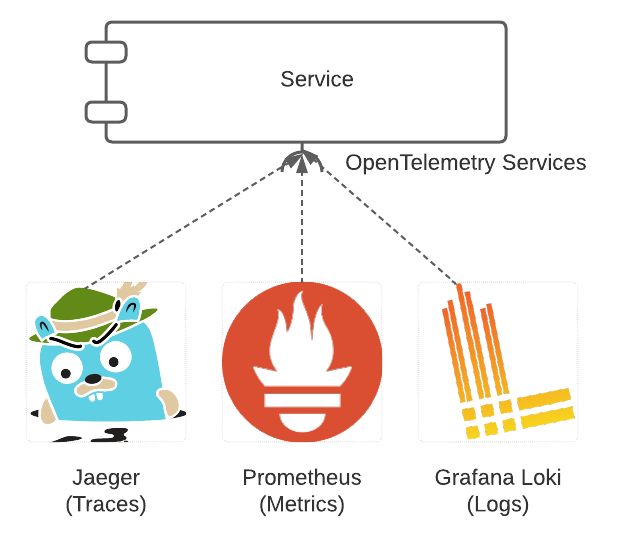
\includegraphics[scale=0.75]{cap_caso-estudio/images/observability-telemetry-collection}
  \caption{Extracto de \emph{logs} de una ejecución habitual.}
  \label{fig:observability-telemetry-collection}
\end{figure}

\subsubsection{Loki: Logs}
Lo primero que queremos ver es cómo mejorar nuestra estrategia de logging. Lo ideal es añadir identificadores de correlación (el traceID), que nos permita rastrear a través de los distintos servicios una misma traza. Por ejemplo, podemos filtrar a partir de ella para ver todos los detalles de los servicios que intervinieron.

\subsubsection{Jaeger: Trazas distribuidas}

Gracias a las trazas distribuidas, podemos ver todas las actividades por las que pasó una petición. En nuestro caso, podemos ver por todos los estados por los que paso.

\subsubsection{Prometheus: Métricas}


\subsubsection{Grafana: Visualización}

Desarrollamos un panel de monitorización con Grafana. Esto nos permitía consultar en un solo lugar las métricas, los logs y las trazas.

